\section{Fehlerbetrachtung}
\label{sec:fehler}


\begin{figure}[h!]
	\begin{center}
		\resizebox{0.8\textwidth}{!}{
			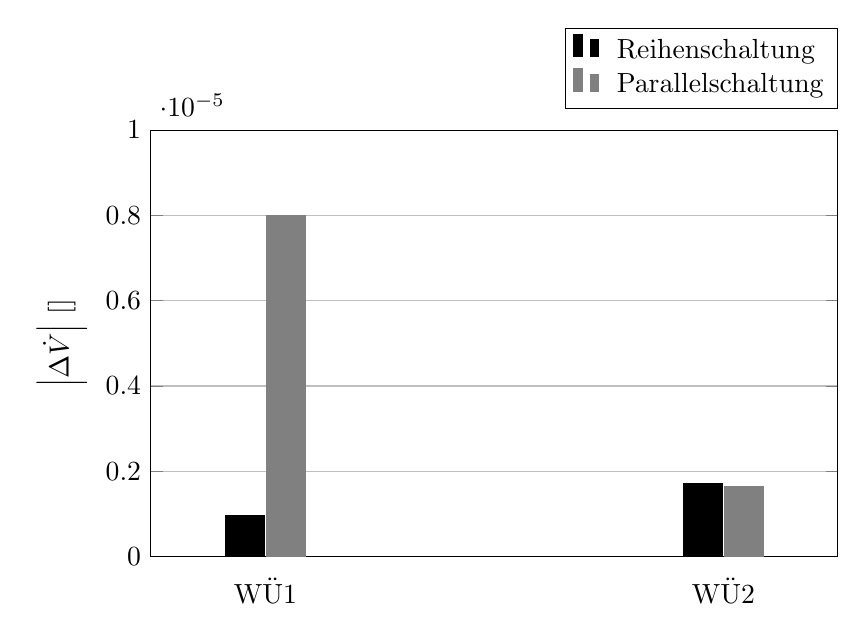
\begin{tikzpicture}
			\begin{axis}[
			width  = 0.85*\textwidth,
			height = 7cm,
			major x tick style = transparent,
			ybar=2*\pgflinewidth,
			bar width=14pt,
			ymajorgrids = true,
			ylabel = {$\left|\Delta \dot{V}\right|\, \left[\si{\cmt\per \second}\right]$},
			symbolic x coords={WÜ1,WÜ2},
			xtick = data,
			%scaled y ticks = false,
			enlarge x limits=0.25,
			ymin=0,
			ymax=0.00001,
			legend cell align=left,
			legend style={
				at={(1,1.05)},
				anchor=south east,
				column sep=1ex
			}
			]
			%Reihenschaltung
			\addplot[style={black,fill=black,mark=none}]
			coordinates {(WÜ1, 9.7E-07) (WÜ2,1.71E-06)};
			
			%Paralaleschaltung
			\addplot[style={gray,fill=gray,mark=none}]
			coordinates {(WÜ1,8.00E-06) (WÜ2,1.64E-06)};
			
			
			\legend{Reihenschaltung, Parallelschaltung}
			\end{axis}
			\end{tikzpicture}
		}
		\caption{Grafischer Vergleich der Korrekturvolumenströme}
		\label{dia:korrrek}
	\end{center}
\end{figure}
\FloatBarrier